\documentclass[tikz,border=5pt]{standalone}
\usepackage{tikz}
\usetikzlibrary{decorations.pathreplacing}

\begin{document}
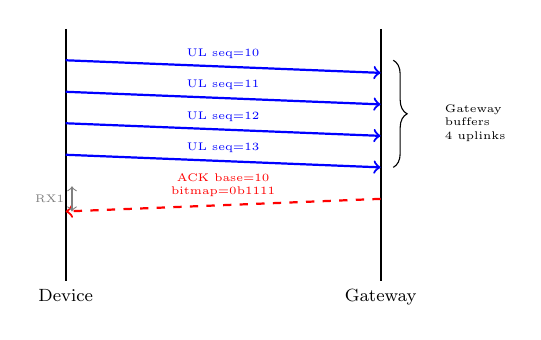
\begin{tikzpicture}[scale=0.8, transform shape]
% Timeline
\draw[thick] (0,4) -- (0,0) node[below, font=\footnotesize] {Device};
\draw[thick] (5,4) -- (5,0) node[below, font=\footnotesize] {Gateway};

% Uplinks
\draw[->, blue, thick] (0,3.5) -- node[above, font=\tiny] {UL seq=10} (5,3.3);
\draw[->, blue, thick] (0,3.0) -- node[above, font=\tiny] {UL seq=11} (5,2.8);
\draw[->, blue, thick] (0,2.5) -- node[above, font=\tiny] {UL seq=12} (5,2.3);
\draw[->, blue, thick] (0,2.0) -- node[above, font=\tiny] {UL seq=13} (5,1.8);

% Aggregated ACK
\draw[->, red, thick, dashed] (5,1.3) -- node[above, font=\tiny, align=center] {ACK base=10\\bitmap=0b1111} (0,1.1);

% Annotations
\node[font=\tiny, align=left] at (6.5,2.5) {Gateway\\buffers\\4 uplinks};
\draw[decorate, decoration={brace, amplitude=5pt}] (5.2,3.5) -- (5.2,1.8) node[midway, right, xshift=3pt, font=\tiny] {};

% RX Window
\draw[<->, gray] (0.1,1.5) -- (0.1,1.1) node[midway, left, font=\tiny] {RX1};

\end{tikzpicture}
\end{document}
